\chapter{ Giới thiệu \& Mục tiêu dự án}
\section{Giới thiệu về Distributed File System (DFS)}

\subsection{Khái niệm DFS}

Distributed File System (Hệ thống phân tán tệp) là một công nghệ cho phép tổ chức và quản lý các tài nguyên lưu trữ phân tán trên nhiều máy chủ vật lý khác nhau, nhưng được trình bày cho người dùng như một cấu trúc thư mục thống nhất và tập trung.

DFS trong môi trường Windows Server bao gồm hai thành phần chính:

\begin{itemize}
    \item \textbf{DFS Namespace:} Cung cấp không gian tên ảo hóa, cho phép người dùng truy cập tài nguyên thông qua một đường dẫn UNC duy nhất (ví dụ: \texttt{\textbackslash\textbackslash detai07.com\textbackslash Public}), mà không cần biết vị trí vật lý của dữ liệu.
    
    \item \textbf{DFS Replication (DFSR):} Công nghệ sao chép dữ liệu đa chủ (multi-master), tự động đồng bộ hóa nội dung giữa các máy chủ thành viên, đảm bảo tính nhất quán và khả dụng cao của dữ liệu.
\end{itemize}

\subsection{Lợi ích của DFS trong môi trường doanh nghiệp}

\begin{enumerate}
    \item \textbf{Tính sẵn sàng cao (High Availability):} Khi một file server gặp sự cố, người dùng tự động được chuyển sang server dự phòng mà không bị gián đoạn dịch vụ.
    
    \item \textbf{Tối ưu hóa truy cập theo địa lý (Site-Aware Access):} Người dùng tự động được kết nối đến file server gần nhất dựa trên cấu trúc AD Sites and Services, giảm độ trễ mạng và cải thiện hiệu suất.
    
    \item \textbf{Đơn giản hóa quản lý:} Thay vì phải nhớ nhiều đường dẫn UNC khác nhau (\texttt{\textbackslash\textbackslash FS1\textbackslash Share1}, \texttt{\textbackslash\textbackslash FS2\textbackslash Share2}), người dùng chỉ cần truy cập một namespace duy nhất.
    
    \item \textbf{Cân bằng tải (Load Balancing):} DFS phân phối yêu cầu truy cập đến nhiều target, giảm tải cho từng server riêng lẻ.
    
    \item \textbf{Khả năng mở rộng (Scalability):} Có thể dễ dàng thêm file server mới vào hệ thống mà không làm gián đoạn dịch vụ hoặc thay đổi đường dẫn truy cập của người dùng.
\end{enumerate}

\subsection{Các thành phần chính trong kiến trúc DFS}

\begin{itemize}
    \item \textbf{Namespace Root:} Điểm gốc của không gian tên DFS (ví dụ: \texttt{\textbackslash\textbackslash detai07.com\textbackslash Public}). Có hai loại namespace:
    \begin{itemize}
        \item \textit{Domain-based Namespace:} Metadata được lưu trong Active Directory, cho phép nhiều namespace server và có tính khả dụng cao hơn.
        \item \textit{Stand-alone Namespace:} Metadata được lưu trên một server duy nhất, phù hợp với mô hình đơn giản.
    \end{itemize}
    
    \item \textbf{DFS Folder:} Các thư mục logic bên trong namespace, đóng vai trò như các liên kết (link) trỏ đến folder target thực tế.
    
    \item \textbf{Folder Target:} Đường dẫn UNC thực tế đến thư mục chia sẻ trên file server (ví dụ: \texttt{\textbackslash\textbackslash FS1\textbackslash DFS\_Public}).
    
    \item \textbf{Replication Group:} Tập hợp các server tham gia vào quá trình sao chép dữ liệu.
    
    \item \textbf{Replicated Folder:} Thư mục vật lý trên mỗi server thành viên được đồng bộ hóa thông qua DFSR.
\end{itemize}

\section{Cơ sở lý thuyết}

\subsection{Active Directory Domain Services (AD DS)}

Active Directory là dịch vụ thư mục của Microsoft, cung cấp các chức năng:

\begin{itemize}
    \item \textbf{Xác thực tập trung:} Quản lý tài khoản người dùng, nhóm và máy tính trong domain.
    \item \textbf{Chính sách bảo mật:} Áp dụng Group Policy để cấu hình và quản lý hệ thống.
    \item \textbf{Phân quyền tài nguyên:} Kiểm soát truy cập dựa trên vai trò (RBAC).
\end{itemize}

Trong đồ án này, AD DS được triển khai trên máy chủ DC01 với domain \texttt{detai07.com}, cung cấp nền tảng xác thực cho toàn bộ hệ thống.

\subsection{Domain Name System (DNS)}

DNS chịu trách nhiệm phân giải tên miền thành địa chỉ IP. Trong môi trường DFS:

\begin{itemize}
    \item Phân giải domain name (\texttt{detai07.com}) thành địa chỉ IP của Domain Controller.
    \item Hỗ trợ DFS namespace trong việc xác định vị trí các file server.
    \item Cung cấp SRV records cho các dịch vụ AD DS.
\end{itemize}

DNS được cài đặt tích hợp trên DC01, đảm bảo độ tin cậy và hiệu suất cao.

\subsection{AD Sites and Services}

AD Sites and Services là công cụ quản lý cấu trúc vật lý của mạng trong Active Directory, cho phép:

\begin{itemize}
    \item \textbf{Định nghĩa Site:} Nhóm các subnet thuộc cùng một vị trí địa lý với kết nối tốc độ cao.
    \item \textbf{Site Link:} Kết nối giữa các site, xác định chi phí (cost) và lịch trình sao chép.
    \item \textbf{Site-Aware Service:} DFS sử dụng thông tin site để chuyển hướng client đến file server gần nhất.
\end{itemize}

Trong đồ án, hai site được tạo:
\begin{itemize}
    \item \textbf{HCM Site:} Subnet 192.168.10.0/24
    \item \textbf{HN Site:} Subnet 192.168.20.0/24
\end{itemize}

\subsection{DFS Replication Protocol}

DFSR sử dụng thuật toán Remote Differential Compression (RDC) để tối ưu hóa băng thông:

\begin{itemize}
    \item Chỉ sao chép các khối dữ liệu thay đổi, không sao chép toàn bộ file.
    \item Hỗ trợ nén dữ liệu trong quá trình truyền tải.
    \item Cơ chế giải quyết xung đột: Last Writer Wins (người ghi cuối cùng thắng).
\end{itemize}

DFSR hoạt động theo mô hình \textit{multi-master replication}, cho phép thay đổi dữ liệu trên bất kỳ server nào và tự động đồng bộ đến các server còn lại.

\subsection{NTFS Permissions và Share Permissions}

Hai lớp phân quyền được áp dụng:

\begin{enumerate}
    \item \textbf{Share Permissions:} Áp dụng khi truy cập qua mạng (SMB protocol), có ba mức:
    \begin{itemize}
        \item Read
        \item Change
        \item Full Control
    \end{itemize}
    
    \item \textbf{NTFS Permissions:} Áp dụng trực tiếp trên file system, chi tiết hơn với các quyền:
    \begin{itemize}
        \item Read (R)
        \item Write (W)
        \item Modify (M)
        \item Read \& Execute (RX)
        \item Full Control (F)
    \end{itemize}
\end{enumerate}

Quyền hiệu lực cuối cùng là quyền \textit{restrictive nhất} giữa Share và NTFS permissions.

\section{Mô hình mạng và Kiến trúc hệ thống}

\subsection{Tổng quan kiến trúc}

Hệ thống được thiết kế theo mô hình \textit{multi-site enterprise network}, mô phỏng một tổ chức có hai chi nhánh tại Hà Nội và Thành phố Hồ Chí Minh, kết nối qua router. Kiến trúc này đảm bảo:

\begin{itemize}
    \item Khả năng mở rộng theo chiều ngang (horizontal scaling)
    \item Tính sẵn sàng cao (high availability)
    \item Tối ưu hóa hiệu suất truy cập dựa trên vị trí địa lý
\end{itemize}

\subsection{Sơ đồ mạng}

\begin{figure}[H]
    \centering
    \includegraphics[width=1\linewidth]{media/mo_hinh_qtm_.png}
    \caption{Mô hình mạng}
    \label{fig:mo_hinh_qtm_}
\end{figure}

\subsection{Bảng phân bổ địa chỉ IP}

\subsubsection{Site HCM (192.168.10.0/24)}

\begin{table}[H]
\centering
\begin{tabularx}{\textwidth}{|l|l|X|}
\hline
\textbf{Thiết bị} & \textbf{Địa chỉ IP} & \textbf{Vai trò} \\ \hline
DC01 & 192.168.10.10 & Domain Controller, DNS Server, DFS Namespace Server \\ \hline
FS1 & 192.168.10.20 & File Server (Primary Target), DFS Replication Member \\ \hline
CLIENT1 & 192.168.10.30 & Windows Client để kiểm thử (Site HCM) \\ \hline
ROUTER-VM (NIC1) & 192.168.10.1 & Default Gateway cho site HCM \\ \hline
\end{tabularx}
\caption{Bảng phân bổ IP - Site HCM}
\label{tab:ip-hcm}
\end{table}

\subsubsection{Site HN (192.168.20.0/24)}

\begin{table}[H]
\centering
\begin{tabularx}{\textwidth}{|l|l|X|}
\hline
\textbf{Thiết bị} & \textbf{Địa chỉ IP} & \textbf{Vai trò} \\ \hline
FS2 & 192.168.20.20 & File Server (Secondary Target), DFS Replication Member \\ \hline
CLIENT2 & 192.168.20.30 & Windows Client để kiểm thử (Site HN) \\ \hline
ROUTER-VM (NIC2) & 192.168.20.1 & Default Gateway cho site HN \\ \hline
\end{tabularx}
\caption{Bảng phân bổ IP - Site HN}
\label{tab:ip-hn}
\end{table}

\subsection{Giải thích lựa chọn địa chỉ IP}

\subsubsection{Lý do chọn dải địa chỉ Private Class C}

Địa chỉ IP được chọn thuộc dải \textit{Private IPv4} theo RFC 1918:
\begin{itemize}
    \item 192.168.10.0/24 (HCM Site)
    \item 192.168.20.0/24 (HN Site)
\end{itemize}

\textbf{Ưu điểm:}
\begin{enumerate}
    \item \textbf{Không xung đột với Internet:} Địa chỉ private không thể định tuyến trực tiếp trên Internet, đảm bảo an toàn.
    \item \textbf{Tiết kiệm địa chỉ công cộng:} Không cần sử dụng địa chỉ public IP cho mạng nội bộ.
    \item \textbf{Dễ nhớ và quản lý:} Cấu trúc đơn giản, phù hợp với môi trường lab và doanh nghiệp vừa và nhỏ.
\end{enumerate}

\subsubsection{Subnet Mask /24 (255.255.255.0)}

Subnet mask /24 cung cấp:
\begin{itemize}
    \item 254 địa chỉ host khả dụng (192.168.x.1 đến 192.168.x.254)
    \item Đủ lớn cho một chi nhánh vừa và nhỏ
    \item Dễ tính toán và troubleshoot
\end{itemize}

\subsubsection{Quy tắc đánh địa chỉ IP}

\begin{enumerate}
    \item \textbf{.1:} Dành cho Gateway (Router)
    \begin{itemize}
        \item 192.168.10.1 (HCM Gateway)
        \item 192.168.20.1 (HN Gateway)
    \end{itemize}
    
    \item \textbf{.10:} Dành cho Infrastructure Servers (DC, DNS)
    \begin{itemize}
        \item 192.168.10.10 (DC01)
    \end{itemize}
    
    \item \textbf{.20 - .29:} Dành cho File Servers
    \begin{itemize}
        \item 192.168.10.20 (FS1)
        \item 192.168.20.20 (FS2)
    \end{itemize}
    
    \item \textbf{.30 - .254:} Dành cho Client và các thiết bị khác
    \begin{itemize}
        \item 192.168.10.30 (CLIENT1)
        \item 192.168.20.30 (CLIENT2)
    \end{itemize}
\end{enumerate}

Quy tắc này giúp:
\begin{itemize}
    \item Dễ dàng xác định vai trò của thiết bị chỉ bằng địa chỉ IP
    \item Đơn giản hóa việc lập kế hoạch mở rộng
    \item Tối ưu cho việc tạo access list và firewall rules
\end{itemize}

\subsection{Cấu hình DNS và Default Gateway}

\subsubsection{DNS Configuration}

Tất cả các máy trong domain đều trỏ DNS về DC01:

\begin{table}[H]
\centering
\begin{tabular}{|l|l|}
\hline
\textbf{Thiết bị} & \textbf{DNS Server} \\ \hline
DC01 & 192.168.10.10 (local) \\ \hline
FS1, CLIENT1 & 192.168.10.10 \\ \hline
FS2, CLIENT2 & 192.168.10.10 \\ \hline
\end{tabular}
\caption{Cấu hình DNS}
\end{table}

\textbf{Lý do:} DC01 là DNS server duy nhất chứa zone \texttt{detai07.com}, đảm bảo phân giải tên chính xác cho toàn bộ domain.

\subsubsection{Default Gateway Configuration}

\begin{table}[h]
\centering
\begin{tabular}{|l|l|}
\hline
\textbf{Thiết bị} & \textbf{Default Gateway} \\ \hline
DC01, FS1, CLIENT1 & 192.168.10.1 \\ \hline
FS2, CLIENT2 & 192.168.20.1 \\ \hline
ROUTER-VM & Không cần (directly connected) \\ \hline
\end{tabular}
\caption{Cấu hình Default Gateway}
\end{table}

\textbf{Lý do:} Router có hai NIC trực tiếp kết nối với cả hai subnet, nên không cần default gateway. Các thiết bị khác cần gateway để giao tiếp giữa hai site.

\subsection{Sơ đồ kiến trúc DFS}

\begin{figure}[H]
    \centering
    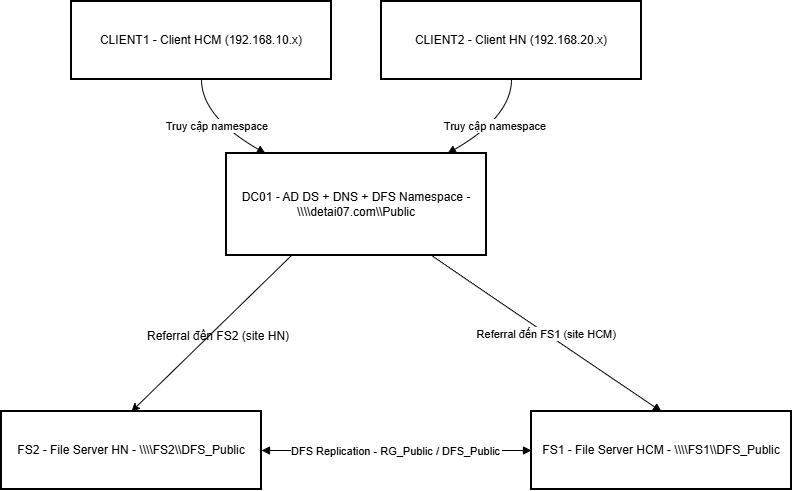
\includegraphics[width=1\linewidth]{media/so_do_kien_truc (1).png}
    \caption{Sơ đồ kiến trúc}
    \label{fig:so_do_kien_truc}
\end{figure}

\section{Chuẩn bị môi trường triển khai}
\subsection{Cấu hình Virtual Machine}

\begin{table}[h]
\centering
\begin{tabularx}{\textwidth}{|l|c|c|c|X|}
\hline
\textbf{VM} & \textbf{vCPU} & \textbf{RAM} & \textbf{Disk} & \textbf{Network Adapter} \\ \hline
DC01 & 2 & 4GB & 60GB & VMnet10 \\ \hline
FS1 & 2 & 4GB & 100GB & VMnet10 \\ \hline
FS2 & 2 & 4GB & 100GB & VMnet11 \\ \hline
ROUTER-VM & 2 & 2GB & 40GB & VMnet10 + VMnet11 \\ \hline
CLIENT1 & 2 & 4GB & 60GB & VMnet10 \\ \hline
CLIENT2 & 2 & 4GB & 60GB & VMnet11 \\ \hline
\end{tabularx}
\caption{Cấu hình Virtual Machine}
\end{table}

\subsection{Cấu hình Virtual Network trong VMware}

\subsubsection{Tạo mạng ảo VMnet10 (HCM Site)}

\begin{lstlisting}[language=bash]
Network Name: VMnet10
Type: Host-only
Subnet IP: 192.168.10.0
Subnet Mask: 255.255.255.0
DHCP: Disabled
\end{lstlisting}

\textbf{Mục đích:} Tạo mạng LAN cô lập cho site HCM

\subsubsection{Tạo mạng ảo VMnet11 (HN Site)}

\begin{lstlisting}[language=bash]
Network Name: VMnet11
Type: Host-only
Subnet IP: 192.168.20.0
Subnet Mask: 255.255.255.0
DHCP: Disabled
\end{lstlisting}

\textbf{Mục đích:} Tạo mạng LAN riêng biệt cho site HN, mô phỏng chi nhánh tại Hà Nội

\begin{figure}[H]
    \centering
    \includegraphics[width=1\linewidth]{media/gan_vmnet.png}
    \caption{Tạo mạng ảo cho 2 site}
    \label{fig:gan_vmnet}
\end{figure}
\subsubsection{Gán Network Adapter}

\begin{table}[H]
\centering
\begin{tabular}{|l|l|}
\hline
\textbf{Virtual Machine} & \textbf{Network Adapter} \\ \hline
DC01 & VMnet10 \\ \hline
FS1 & VMnet10 \\ \hline
CLIENT1 & VMnet10 \\ \hline
FS2 & VMnet11 \\ \hline
CLIENT2 & VMnet11 \\ \hline
ROUTER-VM & Adapter 1: VMnet10, Adapter 2: VMnet11 \\ \hline
\end{tabular}
\caption{Bảng gán Network Adapter}
\end{table}

\textbf{Lưu ý quan trọng:} ROUTER-VM phải có 2 NIC để kết nối cả hai subnet, đóng vai trò gateway và routing giữa hai site.
